% Options for packages loaded elsewhere
% Options for packages loaded elsewhere
\PassOptionsToPackage{unicode}{hyperref}
\PassOptionsToPackage{hyphens}{url}
\PassOptionsToPackage{dvipsnames,svgnames,x11names}{xcolor}
%
\documentclass[
  spanish,
  11pt,
  letterpaper,
  DIV=11,
  numbers=noendperiod]{scrartcl}
\usepackage{xcolor}
\usepackage[left=3cm,right=3cm,top=3cm,bottom=3cm]{geometry}
\usepackage{amsmath,amssymb}
\setcounter{secnumdepth}{-\maxdimen} % remove section numbering
\usepackage{iftex}
\ifPDFTeX
  \usepackage[T1]{fontenc}
  \usepackage[utf8]{inputenc}
  \usepackage{textcomp} % provide euro and other symbols
\else % if luatex or xetex
  \usepackage{unicode-math} % this also loads fontspec
  \defaultfontfeatures{Scale=MatchLowercase}
  \defaultfontfeatures[\rmfamily]{Ligatures=TeX,Scale=1}
\fi
\usepackage{lmodern}
\ifPDFTeX\else
  % xetex/luatex font selection
\fi
% Use upquote if available, for straight quotes in verbatim environments
\IfFileExists{upquote.sty}{\usepackage{upquote}}{}
\IfFileExists{microtype.sty}{% use microtype if available
  \usepackage[]{microtype}
  \UseMicrotypeSet[protrusion]{basicmath} % disable protrusion for tt fonts
}{}
\makeatletter
\@ifundefined{KOMAClassName}{% if non-KOMA class
  \IfFileExists{parskip.sty}{%
    \usepackage{parskip}
  }{% else
    \setlength{\parindent}{0pt}
    \setlength{\parskip}{6pt plus 2pt minus 1pt}}
}{% if KOMA class
  \KOMAoptions{parskip=half}}
\makeatother
% Make \paragraph and \subparagraph free-standing
\makeatletter
\ifx\paragraph\undefined\else
  \let\oldparagraph\paragraph
  \renewcommand{\paragraph}{
    \@ifstar
      \xxxParagraphStar
      \xxxParagraphNoStar
  }
  \newcommand{\xxxParagraphStar}[1]{\oldparagraph*{#1}\mbox{}}
  \newcommand{\xxxParagraphNoStar}[1]{\oldparagraph{#1}\mbox{}}
\fi
\ifx\subparagraph\undefined\else
  \let\oldsubparagraph\subparagraph
  \renewcommand{\subparagraph}{
    \@ifstar
      \xxxSubParagraphStar
      \xxxSubParagraphNoStar
  }
  \newcommand{\xxxSubParagraphStar}[1]{\oldsubparagraph*{#1}\mbox{}}
  \newcommand{\xxxSubParagraphNoStar}[1]{\oldsubparagraph{#1}\mbox{}}
\fi
\makeatother


\usepackage{longtable,booktabs,array}
\newcounter{none} % for unnumbered tables
\usepackage{calc} % for calculating minipage widths
% Correct order of tables after \paragraph or \subparagraph
\usepackage{etoolbox}
\makeatletter
\patchcmd\longtable{\par}{\if@noskipsec\mbox{}\fi\par}{}{}
\makeatother
% Allow footnotes in longtable head/foot
\IfFileExists{footnotehyper.sty}{\usepackage{footnotehyper}}{\usepackage{footnote}}
\makesavenoteenv{longtable}
\usepackage{graphicx}
\makeatletter
\newsavebox\pandoc@box
\newcommand*\pandocbounded[1]{% scales image to fit in text height/width
  \sbox\pandoc@box{#1}%
  \Gscale@div\@tempa{\textheight}{\dimexpr\ht\pandoc@box+\dp\pandoc@box\relax}%
  \Gscale@div\@tempb{\linewidth}{\wd\pandoc@box}%
  \ifdim\@tempb\p@<\@tempa\p@\let\@tempa\@tempb\fi% select the smaller of both
  \ifdim\@tempa\p@<\p@\scalebox{\@tempa}{\usebox\pandoc@box}%
  \else\usebox{\pandoc@box}%
  \fi%
}
% Set default figure placement to htbp
\def\fps@figure{htbp}
\makeatother



\ifLuaTeX
\usepackage[bidi=basic,shorthands=off]{babel}
\else
\usepackage[bidi=default,shorthands=off]{babel}
\fi
\ifLuaTeX
  \usepackage{selnolig} % disable illegal ligatures
\fi


\setlength{\emergencystretch}{3em} % prevent overfull lines

\providecommand{\tightlist}{%
  \setlength{\itemsep}{0pt}\setlength{\parskip}{0pt}}



 


\usepackage{booktabs}
\usepackage{longtable}
\usepackage{array}
\usepackage{multirow}
\usepackage{wrapfig}
\usepackage{float}
\usepackage{colortbl}
\usepackage{pdflscape}
\usepackage{tabularx}
\usepackage{xltabular}
\usepackage{threeparttable}
\usepackage{threeparttablex}
\usepackage[normalem]{ulem}
\usepackage{makecell}
\usepackage{xcolor}
\KOMAoption{captions}{tableheading}
\usepackage{caption}
\captionsetup[table]{position=bottom,labelformat=default,labelsep=colon,name=Tabla}
\captionsetup[figure]{labelformat=default,labelsep=colon,name=Figura}
\usepackage{float}
\floatplacement{figure}{H}
\makeatletter
\@ifpackageloaded{caption}{}{\usepackage{caption}}
\AtBeginDocument{%
\ifdefined\contentsname
  \renewcommand*\contentsname{Tabla de contenidos}
\else
  \newcommand\contentsname{Tabla de contenidos}
\fi
\ifdefined\listfigurename
  \renewcommand*\listfigurename{Listado de Figuras}
\else
  \newcommand\listfigurename{Listado de Figuras}
\fi
\ifdefined\listtablename
  \renewcommand*\listtablename{Listado de Tablas}
\else
  \newcommand\listtablename{Listado de Tablas}
\fi
\ifdefined\figurename
  \renewcommand*\figurename{Figura}
\else
  \newcommand\figurename{Figura}
\fi
\ifdefined\tablename
  \renewcommand*\tablename{Tabla}
\else
  \newcommand\tablename{Tabla}
\fi
}
\@ifpackageloaded{float}{}{\usepackage{float}}
\floatstyle{ruled}
\@ifundefined{c@chapter}{\newfloat{codelisting}{h}{lop}}{\newfloat{codelisting}{h}{lop}[chapter]}
\floatname{codelisting}{Listado}
\newcommand*\listoflistings{\listof{codelisting}{Listado de Listados}}
\makeatother
\makeatletter
\makeatother
\makeatletter
\@ifpackageloaded{caption}{}{\usepackage{caption}}
\@ifpackageloaded{subcaption}{}{\usepackage{subcaption}}
\makeatother
\usepackage{bookmark}
\IfFileExists{xurl.sty}{\usepackage{xurl}}{} % add URL line breaks if available
\urlstyle{same}
\hypersetup{
  pdflang={es-ES},
  colorlinks=true,
  linkcolor={blue},
  filecolor={Maroon},
  citecolor={Blue},
  urlcolor={Blue},
  pdfcreator={LaTeX via pandoc}}


\author{}
\date{}
\begin{document}


\begin{titlepage}
  \centering

  
\includegraphics[width=0.7\textwidth]{logo_facultad.png}\par

  \vspace{3cm}

  {\scshape\Huge Trabajo Práctico de Series de Tiempo \par}

  \vspace{1.5cm}

  {\itshape\LARGE Análisis de muertes por Accidentes Cerebrovasculares (ACV) en Estados Unidos \par}

  \vfill

  {\Large Alumna: Cañizares, María Inés \par}

  \vspace{0.5cm}

  {\Large Licenciatura en Estadística \par}

  \vspace{1cm}

  {\large Año 2026 \par}

\end{titlepage}

\section{Introducción}\label{introducciuxf3n}

El Accidente Cerebrovascular (ACV), conocido popularmente como ``derrame
cerebral'' o ``ataque cerebral'', es una afección médica que ocurre
cuando se interrumpe el flujo de sangre hacia una parte del cerebro, ya
sea porque un vaso sanguíneo se obstruye o porque se rompe. Esta
interrupción hace que las células cerebrales de la zona afectada dejen
de recibir oxígeno y nutrientes, lo que puede provocar daños permanentes
en cuestión de minutos.

El ACV es uno de los principales problemas de salud pública a nivel
mundial. Es una de las principales causas de muerte y, entre quienes
sobreviven, una de las principales causas de discapacidad a largo plazo,
ya que puede dejar secuelas como parálisis, dificultades para hablar o
problemas cognitivos. Además, es una enfermedad estrechamente
relacionada con factores que varían a lo largo del año, como la presión
arterial y la temperatura ambiente, lo que la convierte en un fenómeno
interesante para analizar desde una perspectiva temporal: ¿la cantidad
de muertes por esta causa se mantiene estable a lo largo de los años, o
cambia? ¿Existen ciertas épocas del año donde el riesgo es mayor?

Entender cómo evoluciona la mortalidad por ACV a través del tiempo es
relevante no solo desde el punto de vista médico, sino también para la
planificación de recursos sanitarios: si se pudiera anticipar en qué
meses o períodos aumenta el riesgo, los sistemas de salud podrían
prepararse mejor (por ejemplo, reforzando personal o insumos en los
meses de mayor demanda).

Por este motivo, en este trabajo se analiza la evolución mensual de la
cantidad de muertes por ACV en Estados Unidos entre los años 1999 y
2019, utilizando datos públicos provenientes de CDC WONDER, una base de
datos oficial del gobierno estadounidense que recopila estadísticas
vitales del país. El objetivo es describir el comportamiento de esta
serie a lo largo del tiempo e identificar si existen patrones
recurrentes, como tendencias de largo plazo o variaciones estacionales
asociadas a las distintas épocas del año.

\section{Análisis descriptivo de la serie
temporal}\label{anuxe1lisis-descriptivo-de-la-serie-temporal}

Se presenta la serie temporal de las muertes por ACV mensual en Estados
Unidos durante el período 1999--2018. El gráfico permite visualizar de
manera global cómo se ha comportado la variable en el tiempo.

\begin{figure}

\centering{

\pandocbounded{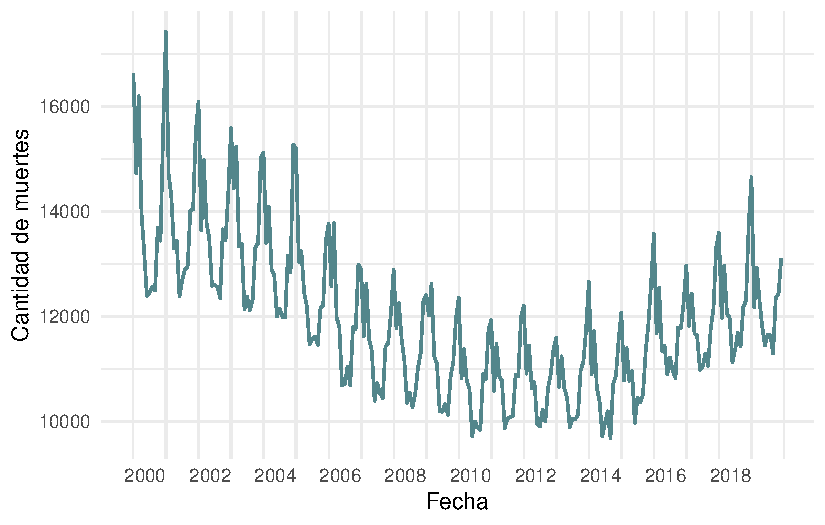
\includegraphics[keepaspectratio]{TP-MInesCañizares_files/figure-pdf/fig-serie-1.pdf}}

}

\caption{\label{fig-serie}Evolución de las muertes mensuales por ACV en
Estados Unidos (1999--2018)}

\end{figure}%

El análisis de la serie muestra que se trata de una variable con
periodicidad mensual, con 12 observaciones por año. En cuanto a la
tendencia, no se observa un comportamiento uniforme a lo largo de todo
el período: entre 1999 y 2010 se registra un descenso sostenido en la
cantidad de muertes, mientras que a partir de 2011 la serie comienza a
mostrar una recuperación progresiva, con un crecimiento que se mantiene
hasta el final del período en 2018. Este patrón refleja un cambio de
dirección en la tendencia, describiendo una forma de ``U'' a lo largo de
los veinte años analizados, lo que indica que la serie no es
estacionaria en media.

Respecto a la estacionalidad, se observa un comportamiento recurrente
año tras año, caracterizado por valores máximos en los meses de invierno
(diciembre, enero y febrero) y valores mínimos en los meses de verano
(junio a septiembre). No se detectaron valores faltantes en el período
estudiado.

Con el fin de profundizar en el análisis de la tendencia y la
variabilidad de la serie, se construyó un gráfico de boxplots anuales
(Figura 2), que permite visualizar la distribución de los datos mes a
mes agrupados por año.

\begin{figure}

\centering{

\pandocbounded{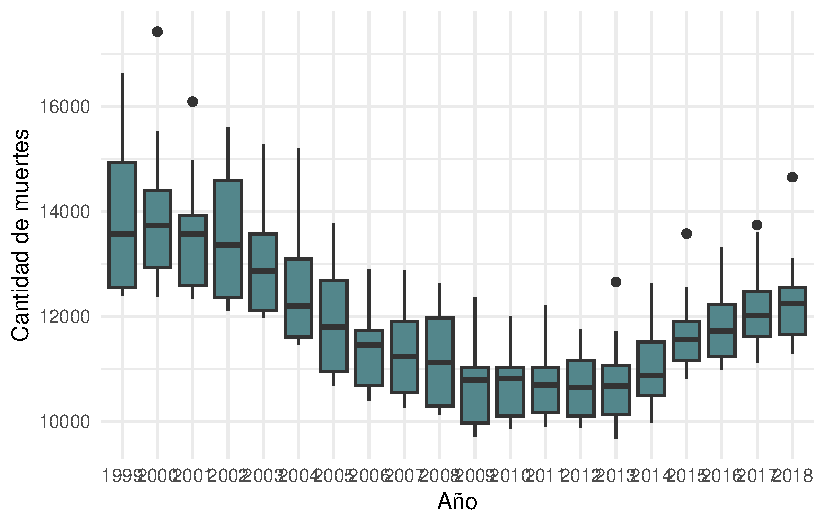
\includegraphics[keepaspectratio]{TP-MInesCañizares_files/figure-pdf/fig-boxplot-1.pdf}}

}

\caption{\label{fig-boxplot}Distribución anual de las muertes por ACV en
Estados Unidos (1999--2018)}

\end{figure}%

Las medianas anuales confirman el mismo patrón en forma de ``U''
descrito anteriormente: descienden desde 1999 hasta aproximadamente
2010-2011, para luego aumentar de manera sostenida hasta 2018.

En cuanto a la dispersión, se observa que la amplitud de las cajas
(rango intercuartílico) no se mantiene constante a lo largo del período:
es mayor en los primeros años de la serie (1999-2003) y en los últimos
(2016-2018), mientras que se reduce notablemente durante los años
centrales (2008-2013). Esta variación en la dispersión acompaña al nivel
general de la serie, lo que sugiere que la variancia no es estable en el
tiempo, es decir, se evidencia heterocedasticidad.

Asimismo, se identifican algunos valores atípicos (outliers) en
determinados años, correspondientes principalmente a meses de invierno
con picos de mortalidad inusualmente altos respecto al resto de las
observaciones de ese mismo año.

Para analizar con mayor detalle el comportamiento estacional de la
serie, se elaboró un gráfico estacional (Figura 3), en el cual se
superponen las observaciones de cada año, ordenadas por mes, con el fin
de comparar la forma del patrón estacional entre los distintos años.

\begin{figure}

\centering{

\pandocbounded{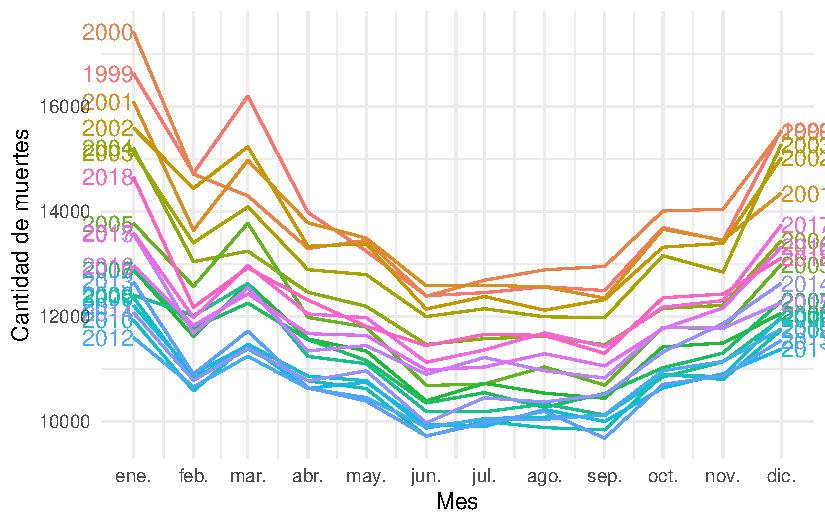
\includegraphics[keepaspectratio]{TP-MInesCañizares_files/figure-pdf/fig-season-1.pdf}}

}

\caption{\label{fig-season}Gráfico estacional de las muertes por ACV en
Estados Unidos (1999--2018)}

\end{figure}%

Se observa que la forma del ciclo estacional se mantiene notablemente
estable a lo largo de todo el período: en todos los años, los valores
más altos se concentran en los meses de diciembre y enero, mientras que
los valores más bajos se registran entre junio y septiembre. Lo que
varía entre los distintos años no es la forma de la curva, sino su nivel
general, lo cual es consistente con la tendencia en forma de ``U''
identificada previamente: las curvas correspondientes a los primeros
años (1999-2003) y a los últimos (2016-2018) se ubican en niveles más
altos, mientras que las curvas de los años centrales (2008-2013) se
ubican en niveles más bajos. En síntesis, el gráfico estacional confirma
la presencia de un patrón estacional anual marcado y persistente en el
tiempo, lo que refuerza la evidencia de no estacionariedad de la serie
observada en los análisis anteriores.

Con el objetivo de aislar el efecto de cada mes en particular a lo largo
de toda la serie, se construyó un gráfico de subseries estacionales
(Figura 4), donde cada panel representa un mes del año y la línea
horizontal indica el promedio histórico de ese mes para todo el período
analizado.

\begin{figure}

\centering{

\pandocbounded{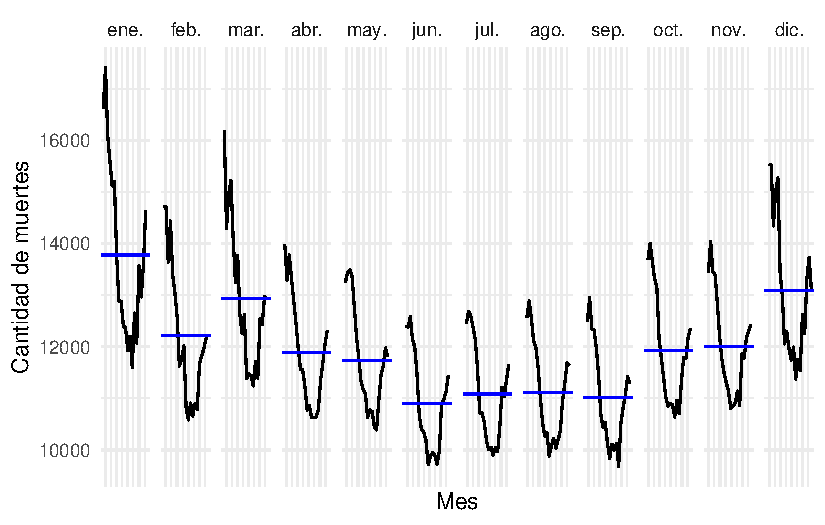
\includegraphics[keepaspectratio]{TP-MInesCañizares_files/figure-pdf/fig-subseries-1.pdf}}

}

\caption{\label{fig-subseries}Gráfico de subseries estacionales de las
muertes por ACV en Estados Unidos (1999--2018)}

\end{figure}%

Este gráfico confirma lo observado en las figuras anteriores: los meses
de diciembre y enero presentan los promedios más altos de mortalidad,
mientras que los meses de junio a septiembre muestran los promedios más
bajos, evidenciando nuevamente el patrón estacional de tipo
invierno-verano. Asimismo, dentro de cada panel se puede apreciar que la
evolución temporal del mes correspondiente también sigue la forma de
``U'' identificada en la tendencia general de la serie, lo que indica
que este comportamiento no solo se da en el nivel agregado, sino que se
repite de manera consistente mes a mes. En conjunto, este gráfico
refuerza la evidencia de un componente estacional fuerte y estable en el
tiempo, que convive con una tendencia no constante a lo largo del
período estudiado.

Finalmente, para contar con una confirmación estadística de las
características observadas en los gráficos anteriores, se calculó la
función de autocorrelación muestral (Figura 5), considerando hasta 36
rezagos.

\begin{figure}

\centering{

\pandocbounded{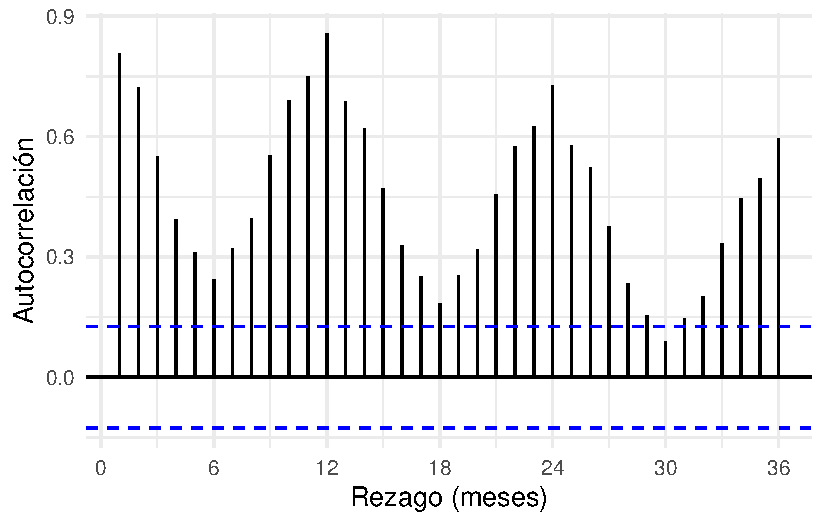
\includegraphics[keepaspectratio]{TP-MInesCañizares_files/figure-pdf/fig-acf-1.pdf}}

}

\caption{\label{fig-acf}Función de autocorrelación de las muertes por
ACV}

\end{figure}%

Se observa un pico de autocorrelación particularmente alto en el rezago
12, que vuelve a repetirse con menor intensidad en los rezagos 24 y 36,
lo cual constituye evidencia formal de la estacionalidad anual detectada
previamente de manera gráfica. Asimismo, se observa que las
autocorrelaciones no decaen rápidamente hacia cero a medida que aumenta
el rezago, sino que lo hacen de forma lenta y sostenida, manteniéndose
por encima de la banda de significancia en la gran mayoría de los
rezagos analizados. Este comportamiento es característico de series no
estacionarias, ya que refleja la presencia de una dependencia de largo
plazo asociada tanto a la tendencia como a la estacionalidad presentes
en la serie. En síntesis, el correlograma confirma de manera formal lo
observado en el análisis gráfico previo, evidenciando que la serie no es
estacionaria ni en media ni en varianza.

Complementando el análisis de la función de autocorrelación, se calculó
también la función de autocorrelación parcial (Figura 6), que permite
identificar la correlación directa entre una observación y su rezago,
eliminando el efecto de los rezagos intermedios.

\begin{figure}

\centering{

\pandocbounded{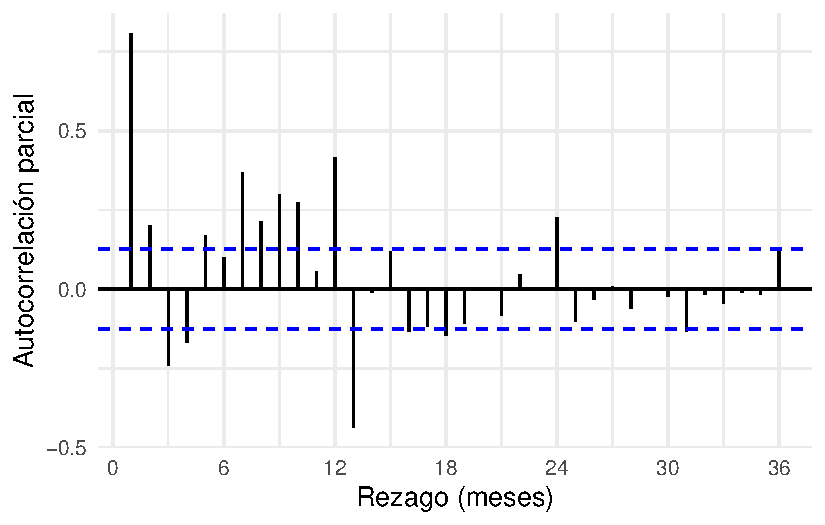
\includegraphics[keepaspectratio]{TP-MInesCañizares_files/figure-pdf/fig-pacf-1.pdf}}

}

\caption{\label{fig-pacf}Función de Autocorrelación Parcial de las
muertes por ACV}

\end{figure}%

Se observa un primer coeficiente muy elevado en el rezago 1 (cercano a
0,8), seguido de varios coeficientes significativos de menor magnitud
entre los rezagos 2 y 10, con signos alternantes. Se destaca además un
coeficiente marcadamente negativo en el rezago 12 (cercano a -0,4), que
resulta notablemente mayor en valor absoluto que el resto de los
coeficientes a partir del rezago 13, los cuales se ubican mayormente
dentro de la banda de significancia o apenas por fuera de ella, salvo un
pico aislado cercano al rezago 24. Este comportamiento sugiere que,
además de la dependencia de corto plazo reflejada en los primeros
rezagos, persiste cierta estructura asociada al componente estacional de
la serie, evidenciada por el coeficiente significativo en el rezago 12.
En conjunto, el correlograma parcial refuerza la idea de que la serie
presenta una estructura de dependencia compleja, consistente con la
presencia simultánea de componentes de corto plazo y de estacionalidad,
lo que confirma nuevamente que la serie no es estacionaria en su forma
original.




\end{document}
